\documentclass[12 pt, a4paper]{article}

\usepackage{geometry}

\geometry{a4paper}

\usepackage[TU]{fontenc}
\usepackage{fourier-otf}

\usepackage{graphicx}

\title{Research and philosophy on transgender people}
\author{Emilia Miki}
\date{April 2023}

\begin{document}

\maketitle

\section{Introduction}

https://www.apa.org/topics/lgbtq/transgender-people-gender-identity-gender-expression 

An American Psychological Association pamphlet that provides general info about terminology, existence of trans people throughout history, difference between sex and gender and so on. 

\section{Debunking Common Anti-Trans Arguments}

https://apsa.org/content/2012-position-statement-attempts-change-sexual-orientation-gender-identity-or-gender 

The American Psychoanalytic Association’s statement on gender identity, in which transness is validated, social stigma against transgender people is cited as a serious cause of harm and ‘reparative therapy’ - attempts to suppress one’s transness and force them to live as the gender they were assigned at birth - is medically invalid. 

\bigskip

https://whatweknow.inequality.cornell.edu/topics/lgbt-equality/what-does-the-scholarly-research-say-about-the-well-being-of-transgender-people/ 

ENORMOUS meta-meta-analysis on transgender people and the effect gender transition has on their mental health 

Of 56 studies, 52 indicated transitioning has a positive effect on the mental health of transgender people and 4 indicated it had mixed or no results. 

ZERO studies indicated gender transitioning has negative results 

The amount of people who detransition is very low (from .3 percent to 3.8 percent), regrets are most likely to result from a lack of social support after transition or poor surgical outcomes using older techniques 

\bigskip

https://publications.aap.org/pediatrics/article-abstract/134/4/696/32932/Young-Adult-Psychological-Outcome-After-Puberty?redirectedFrom=fulltext 

Longitudinal study on the effectiveness of puberty suppression \& sex reassignment surgery on trans individuals in improving mental outcomes 

Unambiguously positive results - results indicate puberty suppression, support of medical professionals \& SRS have markedly beneficial outcomes to trans individuals’ mental health and productivity. 

\bigskip

https://www.ncbi.nlm.nih.gov/pmc/articles/PMC5357259/ 

Meta-analysis covering prior research on trans individuals’ performance in sports and preexisting sports policies concerning trans people 

Findings show there is no consistent or direct research indicating transgender women have an unfair athletic advantage at any stage of their transition. 

Additional findings show most sports policies are not evidence-based and trans individuals experience substantial discrimination from sports institutions. 

\bigskip

https://www.cces.ca/sites/default/files/content/docs/pdf/transgenderwomenathletesandelitesport-ascientificreview-e-final.pdf 

"Evidence directly examining the effect of testosterone suppression as it directly affected trans women’s athletic performance showed no athletic advantage exists after one year of testosterone suppression (Harper, 2015, 2021)" 

https://www.scientificamerican.com/article/beyond-xx-and-xy-the-extraordinary-complexity-of-sex-determination/ 

the study is paywalled 

Scientific American graphic describing the many characteristics which factor into one's sexual identity.

Helpful in indicating the ambiguous and bimodal nature of sex/responding to people who believe it’s as simple as XX/XY 

\begin{figure}[ht]
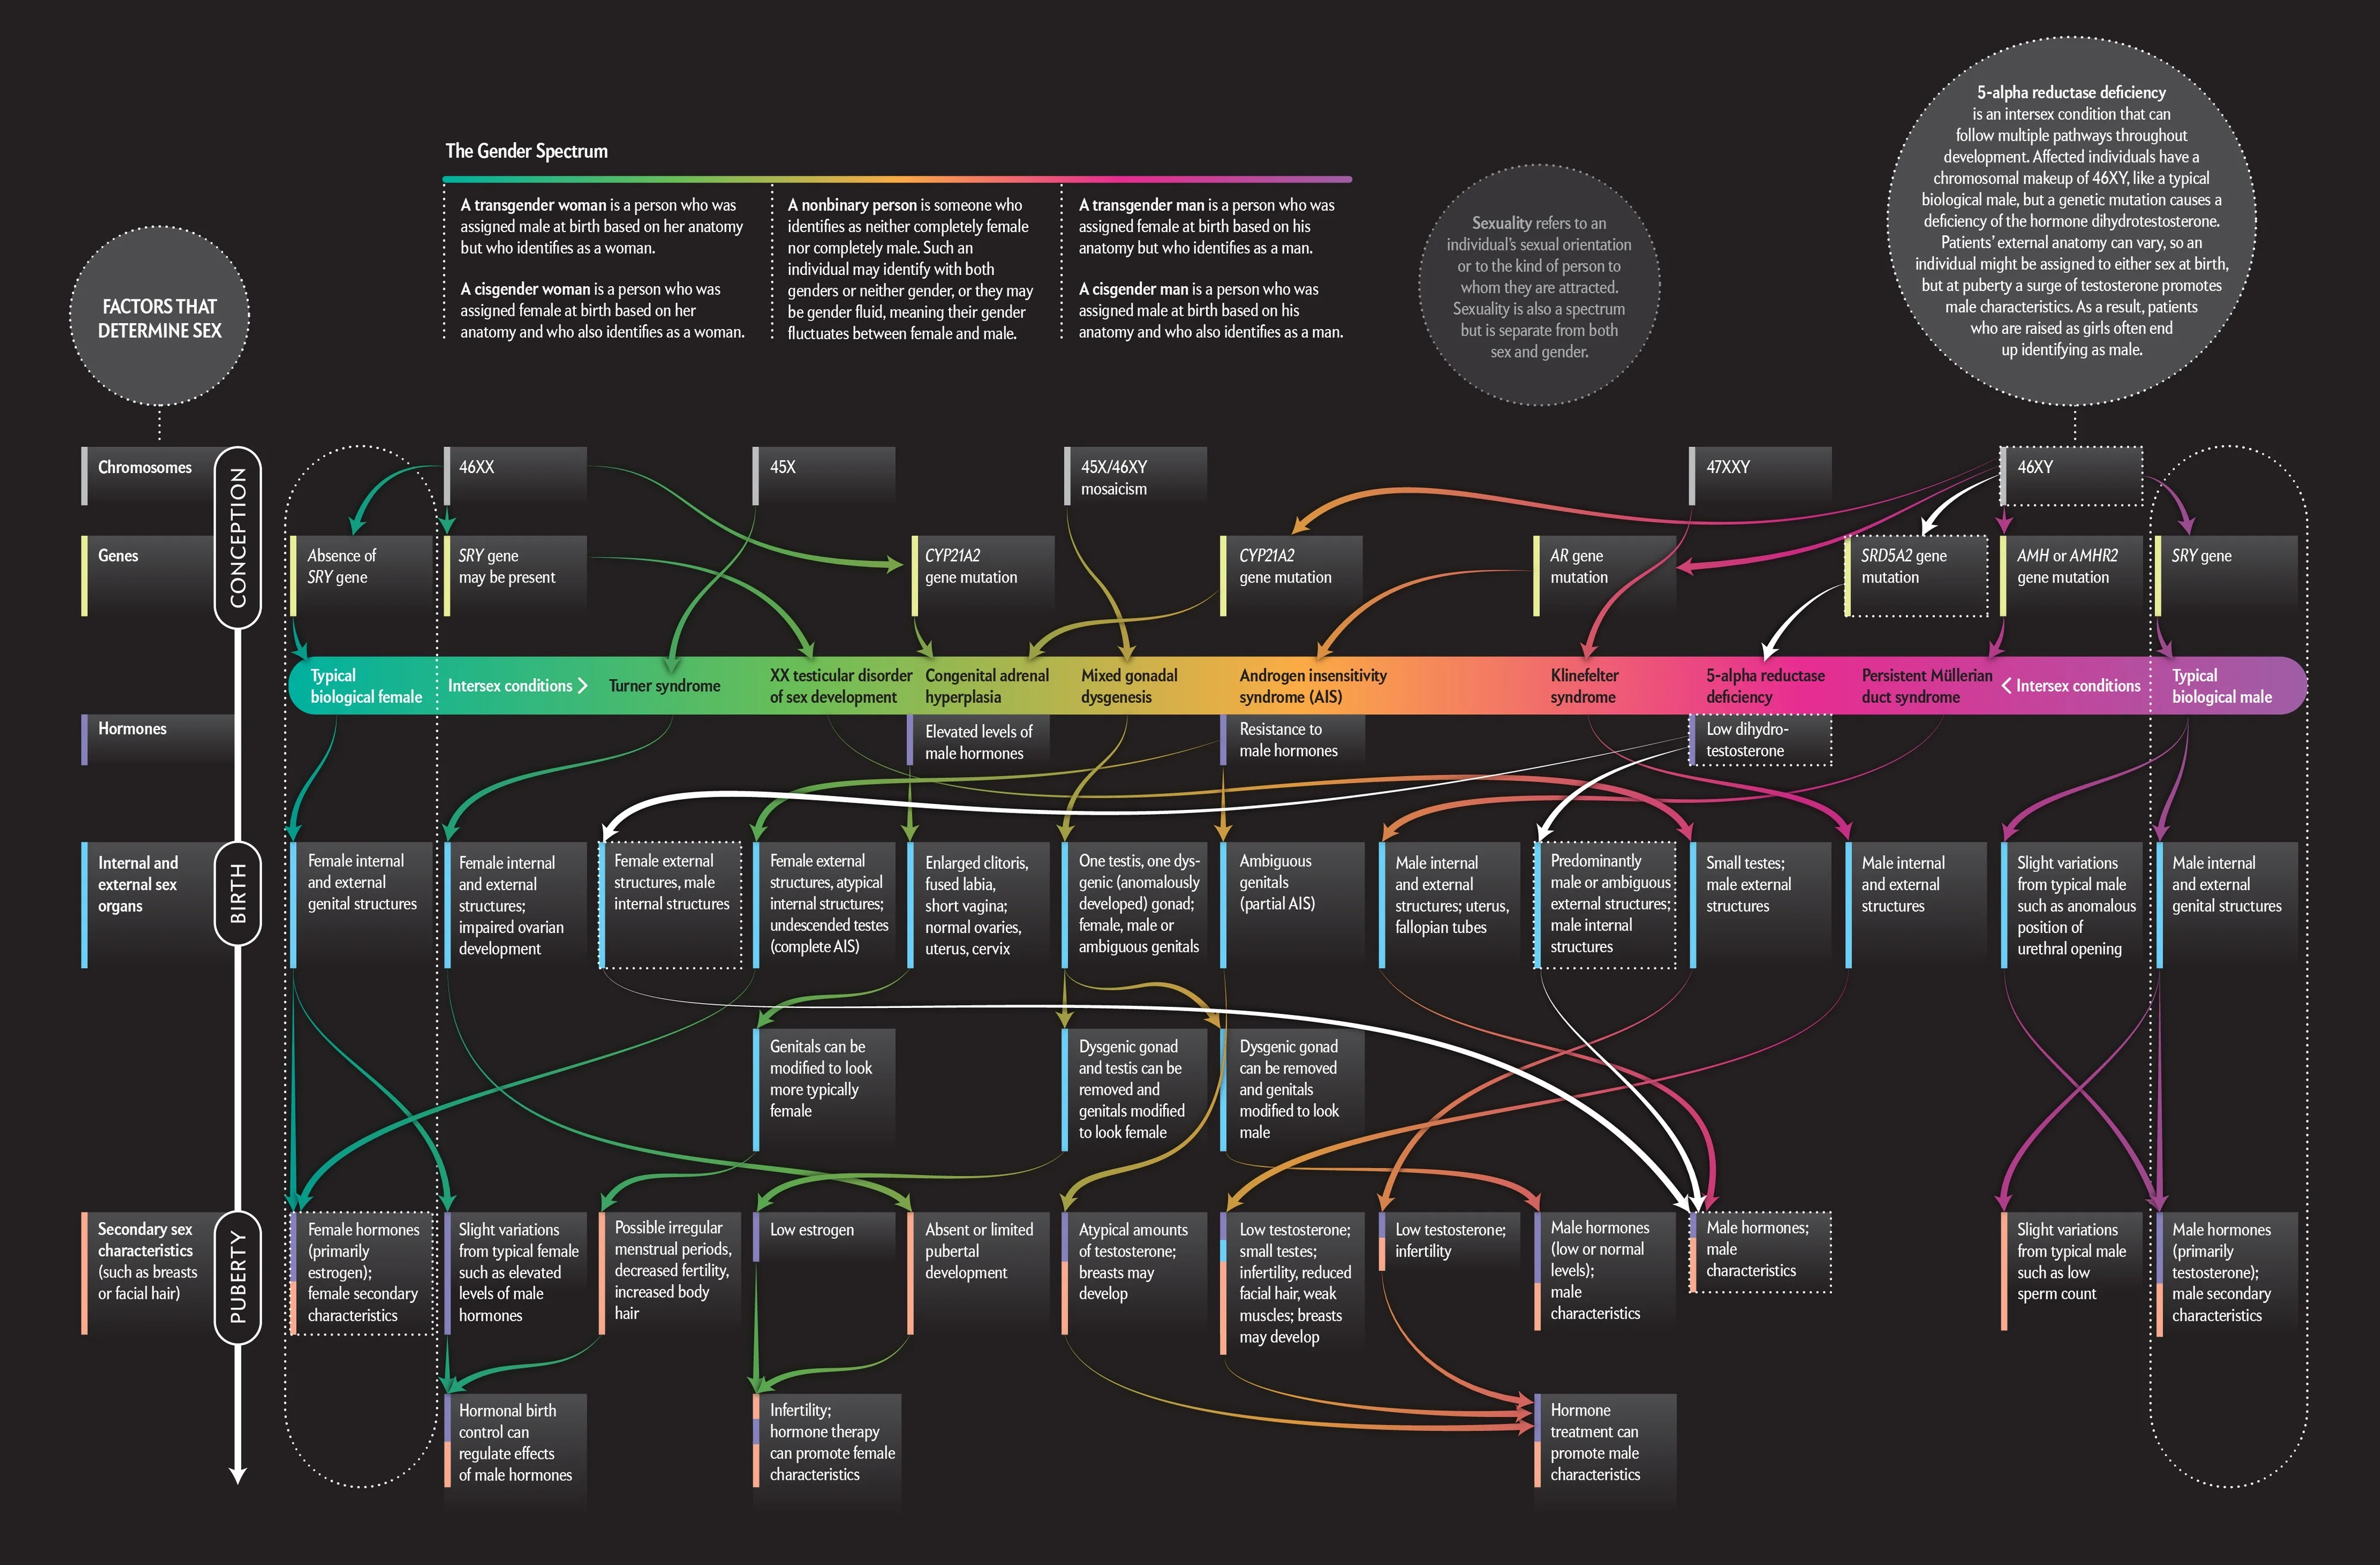
\includegraphics[width=\textwidth]{beyond-xx-and-xy.png}
\caption{Credit: Pitch Interactive and Amanda Montañez; Source: Research by Amanda Hobbs; Expert review by Amy Wisniewski University of Oklahoma Health Sciences Center}
\end{figure}

\bigskip

https://www.researchgate.net/publication/328057475\_Untangling\_the\_Gordian\_Knot\_of\_Human\_Sexuality\_What\_Is\_the\_Biologic\_Basis\_of\_Variations\_in\_Sexual\_Phenotype

Description of modern scientific attitudes towards human sex. 

“The view that the world’s population can be separated into a clearly defined dyadic unit of male and female is defunct; not only clinical observations, but molecular biology has established that sexual identity is on a continuum, with an enormous potential for variance” 

\bigskip

https://assets2.hrc.org/files/assets/resources/2018-YouthReport-NoVid.pdf?\_ga=2.134619825.1102244158.1526302453-846000759.1523970534 

2018 LGBTQ Youth Report 

HUGE collection of data concerning difficulties LGBTQ people face 

67\% of LGBTQ youth hear their parents make negative statements about LGBTQ people - rises to 78\% if child is in closet. 

48\% of LGBTQ youth say their family makes them feel bad for their identity 

This pretty much ends the argument right here. 

\bigskip

https://www.ncbi.nlm.nih.gov/pmc/articles/PMC5178031/ 

Broad international study of trans suicide rate (it’s quite high). 

“Gender-based victimization, discrimination, bullying, violence, being rejected by the family, friends, and community; harassment by intimate partner, family members, police and public; discrimination and ill treatment at health-care system are the major risk factors that influence the suicidal behavior among transgender persons”. 

\bigskip

https://transpulseproject.ca/wp-content/uploads/2012/10/Impacts-of-Strong-Parental-Support-for-Trans-Youth-vFINAL.pdf 

Analysis of the ways in which parental support affect elements of disadvantage experienced by transgender youth. 

Most notably, strong parental support decreases the likelihood of a suicide attempt within the past year from 57\% to just 4\%. 

\section{Personal Experience}

There are lots of clues that may indicate to people that they are transgender and don't feel comfortable living as the assigned gender at birth, like dreaming about being the opposite gender, thinking that being the opposite gender is objectively better and that everyone knows that. But usually the scariest stuff begins at puberty, when your body starts to actively change because of sex hormones and if you're trans, to you this will feel like a torture, like there is poison in your body making you into something you don't want to be. It raises anxiety and depression drastically (as shown in studies above) and it's scary to experience.  

That's why in first world countries people use puberty blockers. There are lots of myths about them propagated by transphobes, and here's an article that disproves all of them with actual research: https://www.gendergp.com/puberty-blockers-dangers-harmful-myths/. In general, they work by delaying puberty and giving the patient time to think if they are sure that they are transgender, and when they feel confident that they are transgender, they go on with HRT and experience the desired puberty, or, if they decide they are cisgender, they just stop taking puberty blockers and experience their puberty as usual. Puberty blockers have the added benefit of this has the added benefit of making trans people 100\% indistinguishable from cisgender people due to never their birth-sex puberty and only experiencing the desired sex puberty. Of course, this also has a very good positive effect on their mental health and quality of life later on, as confirmed by studies above. 

Now some general information about HRT (Hormone Replacement Therapy). Male and female humans are exactly the same in every way after conception in the womb of the mother. The same embryo can develop male or female genitals depending on which hormone washes they received in the womb, and they are capable of developing either. And thanks to them being structurally very similar and developed in a very similar way, it is possible to create a vagina with penile inversion surgery that is indistinguishable from a naturally developed one. After birth the hormones begin to work only at puberty. Before that children don't develop any other sexual characteristics and stay androgynous. After puberty, depending on the hormones you have in your body, it will develop sexual characteristics, some of which are reversible and some are not. 

Here's a list of the changes (everything is reversible except if marked otherwise, T – testosterone, E – estrogen): 
\begin{itemize}
\item Voice Drop for T (irreversible), transwomen can still sound perfectly feminine using voice training 
\item Bottom Growth for T, atrophy for E (irreversible) 
\item Cessation of Menstruation for T 
\item Male Pattern Baldness for T 
\item Breast Growth for E (the size is determined by your genes, usually is comparable to your mother's or sister's) (irreversible) 
\item Changes in Body Temperature Placement (less sensitive to cold for T and more sensitive for E) 
\item Changes in Perspiration (more sweat in specific areas for T and distributed sweat over the whole body for E) 
\item Body Odor (stronger and masculine for T, reduced and feminine for E) 
\item Body Hair thicker, in more places and grows faster for T, opposite for E 
\item Thicker and Oilier Skin for T, Skin Softening for E 
\item Increased body flexibility for E and decreased for T 
\item Larger Hands / Feet for T and smaller for E 
\item Thicker and Stronger Nails for T and thinner and lighter for E 
\item Increased Muscle Mass for T and massively decreased musle mass for E 
\item Fat Redistribution
\item Facial Feature Changes 
\item Increased Tolerance of Caffeine, Alcohol, and/or Psychotropics for T and decreased for E 
\item Mental Changes (more/less emotional sensitivity, different types of orgasm) 
\end{itemize}

In general, HRT brings most sexual characteristics and body appearance in close alignment with the desired sex, which also impacts the way you have to be treated by doctors (for example, Male-to-Female trans people don't have to do prostate checks because they can't get prostate cancer, but they have to to breast checks, because they can get breast cancer). 

\section{History, Politics, Philosophy}

Now let's get into some history and politics. Sometimes this might seem unrelated, but it will be used later to tie philosophical ideas into the perception and existence of trans people and other groups of people now and in the past. 

13/50 is a common white supremacist argument that refers to the statistic that despite making up 13 percent of the population, African Americans make up 50 percent of the violent crime in the US. They tie the quality of being violent to the identity of being black and treat it as an essential part of being black. The reality is that black people commit more crime in the US because of systemic discrimination that is still present in society. For example, in the United States, redlining is a discriminatory practice in which services (financial and otherwise) are withheld from potential customers who reside in neighborhoods classified as "hazardous" to investment; these neighborhoods have significant numbers of racial and ethnic minorities, and low-income residents.[2] In the United States, the Fair Housing Act of 1968 was passed to fight the practice of redlining, which is very recently in historical standards. But it doesn't mean that redlining just instantly disappeared. In fact, the fight against it continues today: In May 2015, the U.S. Department of Housing and Urban Development announced that Associated Bank had agreed to a \$200 million settlement over redlining in Chicago and Milwaukee. The three-year HUD observation led to the complaint that the bank purposely rejected mortgage applications from black and Latino applicants. The final settlement required AB to open branches in non-white neighborhoods. 

Redlining led to black people being segregated in poor neighborhoods without economic opportunities, which leads to more crime being commited, gang violence, drug trafficking, which leads to even more people being arrested (because of the drug war, which in itself is a completely failed and strictly harmful policy), which leads to more children who grow up without a father, which leads to even more poverty and crime. This is a feedback loop that won't resolve itself if we just leave everything as is, and redlining is only a single small factor among hundreds, that leads to more crime and poverty among black people. Centuries-long discrimination left it's trace and it won't just magically disappear overnight without action to fight it, but for essentialists it's always easier to ascribe all the problems that disproportionately affect a group of people, to the essence of that group of people. Same thing happens on the other side, too: there are "black liberation" activists who essentialize white people as being inherently dominating, colonizers, exploitative and so on, and their perceived solution for this problem is the same as white nationalists' one: an ethnostate, a complete separation of black and white populations with national borders. In practice to implement this you'll need a civil war or another kind of authoritarian takeover, then deportation and genocide. 

Same thing happened in the past with Irish people, who were considered mentally inferior to the British by the British. This belief originated from the following quote: “. . . found the Irish to have IQs which were not very different from those observed in American negroes, and far below comparable English samples” (Eysenck, 1971, p. 127). There were numerous arguments since the 19th century and now, usually employed by white supremacists, about some races being superior to others in terms of intellect base on some studies that recorded IQ differences between races. But the scientific consensus is that there is no evidence for a genetic component behind IQ differences between racial groups. Growing evidence indicates that environmental factors, not genetic ones, explain the racial IQ gap. Again, the white supremacists try to essentialize lower average IQ of different races or ethnicities. 

(here we go to the philosophy part, smoothly as fuck) 

In general, you don't need to go far to understand what essentialism leads to. Just ask the main essentialist thinker - Plato. In The Republic, Plato's ideal state was an authoritarian one, segregated into different classes without mixing between them, everything had to be carefully planned according to the ideal vision he laid out and never stray from it, which, of course, requires strict enforcement of these rules by the violent state. Each group had some essential qualities ascribed to it by Plato, there was required a strict hierarchy without questioning those who are above you. In general, it was a proto-fascist ideal. Modern fascists are much less coherent in their ideology, but the basic principles remain the same, and being an essentialist is usually what leads to them at the core. 

The limit of fascist ideology is, of course, the nazis. Here's an interesting fact from history: trans people and LGBTQ+ people were among the first ones to be targeted by the Nazis. Especially contemptuous for them was the Institut für Sexualwissenschaft, which was an early private sexology research institute in Germany from 1919 to 1933. It was the first sexology research center in the world. The institute pioneered research and treatment for various matters regarding gender and sexuality, including gay, transgender, and intersex topics. In addition, it offered various other services to the general public: this included treatment for alcoholism, gynecological examinations, marital and sex counseling, treatment for venereal diseases, and access to contraceptive treatment. It offered education on many of these matters to both health professionals and laypersons.

The Nazi book burnings in Berlin included the archives of the institute. After the Nazis gained control of Germany in the 1930s, the institute and its libraries were destroyed as part of a Nazi government censorship program by youth brigades, who burned its books and documents in the street. 

This is pretty easy to understand after analyzing their ideology. Because of centirues or even millennia-long discrimination of Jewish people by Christians, and because of the Christian prohibition on interest rates, Jews were overrepresented in the german banking system, they were generally more wealthy and educated because of other historical and religious details similar to the interest rate prohibition and because they were frequently expelled from countries for no reason except bigotry, so their natural career choice was to become merchants. Here we have an analogous situation with the described earlier white privilege, the systemic discrimination of black people, race realism and so on. And the nazis' response was analogous – essentialize the attributes associated with Jewish people. And of course, the practical solution of these inequities for the essentialist mind can only be one: to exterminate the group of people whose essence contains these undesirable attributes. 

What about queer people? Well, first of all, trans people basically argue for the ability to move from one gender category to another. Obviously, that is literally impossible for essentialists, because in their minds these categories are immutable and completely distinct, frequently they are also God-given or otherwise religiously justified, and they are not material, but idealist. They are something you can't change by manipulations in the material world. In the case of sexual minorities, for the nazis they seemed to go against the "natural order", which basically stands for the hierarchical order the nazis liked most. Queer people were perceived as political threats, because, obviously, nazis don't like multiplicity of lifestyles and opinions. Essentialism necessarily leads to the idea of enforcing a single lifestyle perceived as "the best one" and suppressing everything that deviates from it. 

You know about the old argument about the ship of Theseus that challenges the simplistic essentialist view. There are lots of other arguments, like the fact that most things in the world, especially in nature, are on a spectrum. You can't find a single objectively correct boundary to draw between two categories when it comes to sex and intersex people, evolution and the point at which one species "becomes" another one, the point at which a white person becomes a black one in the case of race mixing, and so on. And essentialist definitions can ALWAYS be challenged. Plato's ideas about essential qualities of different groups of people will never find anything analogous in reality if you do any statistical research, there are always multiplicities of different qualities in different supposed categories of people, there are always outliers and so on; any definition of what is the essence of a human will fall apart when you consider people with different disabilities, diseases, mutations, people augmented by technology in different ways; any essentialist definition of what is a woman will not hold up to women who were born with chromosome abnormalities, to women who go through menopause, to women who are infertile for some reason, women who have different kinds of anomalies but are still considered women and can't be categorized as men. And if you decide to just create simple definitions for what a man is and what a woman is, and then say that everyone else falls into some "intersex" category – the intersex category will not have an essentialist definition, you won't be able to find the essence of being intersex. Not even saying that those strict definitions of a man and a woman will probably be very impractical in the real world and wouldn't represent what people actually treat as a man and a woman. 

The real world is not essentialist, and treating it as if it is always results in unfounded discrimination, misplaced hatred, incorrect analysis of the causes of different problems, and authoritarian politics that lead to inhuman actions limiting people's freedoms. What's the alternative? Well, the alternative is to recognize that the world is much more complex than we thought and it isn't categorizable. There is no single coherent view of the world that simplifies it down to strictly defined categories and relations, but that doesn't mean that we lost all hope for science and understanding the world better. Actually it's completely the opposite. We can and should acknowledge all differences that exist in the world, and we're no longer tied by the desire to categorize. We can use statistics, different philosophical lens of analysis based on thinking about differences between things instead of their supposed non-existent essence. This doesn't make our worldview worse, it lets us understand the world as it is, more accurately, precisely, more aligned with reality, including all details and nuance present in it. 

First, you can read Wittgenstein, who argued that the meaning of words is best understood as their use within a given language game, and not separately from one another and their external context. Then you can dive into existentialist thinkers, who famously proposed the idea that "existence precedes essence", a profoundly liberating idea for every thinking person. Then you can dive into structuralism. Let me quote some concepts of Saussure's structural linguistics: 

Saussure argued for a distinction between langue (an idealized abstraction of language) and parole (language as actually used in daily life). He argued that a "sign" is composed of a "signified" (signifié, i.e. an abstract concept or idea) and a "signifier" (signifiant, i.e. the perceived sound/visual image). 

Because different languages have different words to refer to the same objects or concepts, there is no intrinsic reason why a specific signifier is used to express a given concept or idea. It is thus "arbitrary." 

Signs gain their meaning from their relationships and contrasts with other signs. As he wrote, "in language, there are only differences 'without positive terms.'"

Structuralism was applied in many sciences and it did make our understanding of the world much better. Of course, you shouldn't stop here. There are critics of structuralism, known as post-structuralists, and their contribution is also worth reading and contemplating upon. If you're curious about the applications of these ideas to feminism and gender studies, you can read thinkers who worked in this issue. What is gender was one of the concepts that were essential categories before being questioned by non-essentialist thinkers, but even now there are different opinions about what it is and what to do with it. There are ideas like gender accelerationism and gender abolitionism, which generalize to identity abolition in general. Philosophers who propose this argue that any socially constructed identity (including race, gender, sexuality and others) is fundamentally just another constraining category you put on yourself and on the world around you, and the only thing that results from it is more people feeling inferior due to not being fully conforming to those categories, more people being discriminated based on them, discouragement of actual free self-expression without trying to conform or replicate any of these identities, and so on. Gender accelerationists argue that the best way to achieve gender abolition is by letting everyone invent their own gender that best describes that person, leading to the concept of gender eventually becoming meaningless and disappearing, because at some point people will just start describing how they feel in their own words without references to any social construct, liberating thought and expression. 

Now let's get into transhumanism, another philosophical concept closely related to trans people. For non-essentialists, transhumanism is what makes us human and it has been with us since the first human figured out how to use tools. When you use a tool, you can feel it being an extension of your hand. When you drive a car, you can feel it accelerating or decelerating, you can feel how big it is, how fast it goes and so on. We have always manipulated the nature around us and extended our own nature with the tools we use. A person with a hammer has different abilities to a person without one. We have used medicine to do the same. Transhumanists, politically, argue that people who push against abortion, against hormone replacement  therapy or anything else, are just reactionaries (read essentialists) who are scared of the latest tech invented to enhance the possibilities of extending human nature. Trans people are living the latest edge of transhumanism, they use modern hormones created by humans to change their biological characteristics in a way more drastic than anything that came before, and it scares some people. Transhumanists also argue that the ability to change your body in whatever way you want is something that should be added as a human right that must be protected, it is a fundamental freedom that humans must be able to enjoy. I tend to agree.  

In the end, I want to offer you a quote from somebody who certainly did not like the ideas of transhumanists much, and then criticize it a bit: 

"When people attempt to rebel against the iron logic of nature, they come into conflict with the very same principles to which they owe their existence as human beings. Their actions against nature must lead to their downfall". 

– Adolf Hitler, Mein Kampf 

So, my objection to this would be, again, essentialism. "Nature" has always been a multiplicity without essence, it is a random ever-changing world of incremental differences, it is unstable and very diverse. Everything that humans have ever felt or done can only be considered natural, because it was in nature. We are part of nature, and everything we do in terms of creating tools, industrializing, manipulating our environment, building – is also natural and something that nature is doing through us. Hitler probably knows this too, but he chooses to include some things in his ideas of what "the natural order" is, add some new ideas from his head to this vision, and exclude some other things (like the fact that homosexuality is also natural and common in other animal species besides humans, too). 

Another point is that nature wasn't created as something fixed, eternal and perfect, it is just a random set of occurences guided by physics. Even if you believe in the christian God, you still can't deny this point, because the first sin of humanity made nature flawed too, which is confirmed by the apostle Paul in the passage: "For the creation was subjected to frustration, not by its own choice, but by the will of the one who subjected it, in hope that the creation itself will be liberated from its bondage to decay and brought into the freedom and glory of the children of God." (Romans 8:19-21). There is even a fallacy taught in every logic course – appeal to nature fallacy. If something is in nature, it doesn't mean that it is good. Most people agree that rape and murder aren't good and should be minimized, but they were certainly common in nature in the past. 

\begin{itemize}
    \item https://en.wikipedia.org/wiki/Essentialism 
    \item https://en.wikipedia.org/wiki/Ludwig\_Wittgenstein 
    \item https://en.wikipedia.org/wiki/Structuralism 
    \item https://en.wikipedia.org/wiki/Post-structuralism 
    \item https://en.wikipedia.org/wiki/Gender\_studies 
    \item https://en.wikipedia.org/wiki/Transhumanism 
\end{itemize}

\end{document}
